\chapter{High-Dimensional Datasets and Tests}
High dimensional datasets are not a very common research topics. In this chapter I will describe some data sources and possible applications of the described algorithm. I also show some interpretations of subspaces in different datasets and some failed approaches of finding them.

This chapter will also compare GraBaSS against ENCLUS, which is described in \cite{enclus}. The main parameters of ENCLUS are named as stated in the paper, so they are $\epsilon$ and $\omega$, but the binning parameter is $\xi$, and describes the number of bins. So the parameter $\vartriangle$ of the ENCLUS paper for a dimension $X$ is $\vartriangle = \frac{\max{X} - \min{X}}{\xi}$. Both algorithms use the same implementation techniques and data backend described in chapter~\ref{chap:implementation}. They are compiled using Clang~3.3 using \texttt{-O3} and \texttt{-ffast-math} flags. Using this optimization, Clang is able to to vectorize some parts of the implementation. This means, that loops can be replaced by a variant that uses SIMD operations, which speeds up the compiled executable. The used TBB has version~4.0.

To get, isolate and preprocess the data I've used some scripts. Because I think open research should not only contain open publications but also open data sources, you can find the scripts and some notes about them online.\footnote{\url{https://github.com/crepererum/GSD}} Should you have some questions, find a bug or want to contribute, feel free to use the issue tracker or file a pull request.

\section{Architecture and Climate}
This data set is a time series that is used to determine, when windows of a building should be opened and when they should closed. To archive this, different metrics are measured at different locations of the builds, e.g.:
\begin{itemize}
	\item light intensity from different directions
	\item wind force and direction
	\item outer and inner air temperature
	\item temperature of the building itself
	\item energy consumption of lighting, ventilation, air conditioner, different consumers in the rooms
	\item CO2 concentration
	\item status of the manual sun protection system and manual opened windows
\end{itemize}

The data set is only available for institute members, so I cannot provide a source. The original data set contains \num{434} dimensions and \num{43896} objects, where the dimensions are the different metrics and the objects are the different points in time. Because the data set contains missing values, it is preprocessed. Dimensions are removed when they contain more then \SI{10}{\percent} missing values. After this step, all objects that still have some cells with missing values are also removed. This cuts the data set down to \num{271} columns and \num{35400} objects.

GraBaSS gets invoked with $t_e = 0.15$, $t_n = 0.65$ and $d = 3$. It tends to group metrics of subsystems together, that have some logical dependency, e.g.:
\begin{itemize}
	\item volume of supply air, volume of used air, energy consumption for both systems
	\item air temperature in different parts of the building
	\item temperature of different parts of building itself
	\item temperature of some parts of the building itself and temperature of some rooms
	\item CO2 concentration at some measure station and temperature of some parts of the building
	\item number of persons in a room, manual window state and volume of supply air and used air
\end{itemize}

The algorithm also produces some less logical results, as the CO2 concentration at some points and the temperature of some parts of the building, but this cases are very rare, so they might be as anomalies.

ENCLUS has a problem with this data set, because it contains some outliers. Some dimensions contains only small data from \num{0.1} to \num{0.2}, but some measures are described by values of \num{100} and more. Because ENCLUS uses an equi-width descretizer and calculates entropy values on this discrete values, it tries to join all dimensions with this kind of outliers. It also destroys some useful subspaces, if you are able to get some results. Because of the size of the data set, the number of affected dimensions and the size of the subspace is also large. This increases calculation of ENCLUS to calculate the results, so it does not finish within hours.

\section{Drug Database}
A source of high dimensional data is the list of ingredients of drugs. They collect important information about common combination of substances because one ingredient requires another, e.g. alcohol is a solvent for many chemicals. Common combinations can also be formed by combined substances that are used in drugs because manufactures produce them as a base for their product or because they act as a reseller for premixed drugs. The data set also contains information about chemicals that are never used together because they react with each other or because it does not make sense in terms of usability.

I hoped to find some public drug data bases containing drugs registered in Germany or in the EU. But this was not the case. Either they were only usable via a very limited interface or it would cost me a enormous amount of money to buy a license. Since the open data movement in USA has a very long tradition, it was easy to find an American drug database, that is easy to parse and provides a huge data collection.\footnote{\url{http://dailymed.nlm.nih.gov/dailymed/downloadLabels.cfm}} The entire data set contains \num{24094} drugs and \num{4139} possible ingredients. Figure~\ref{fig:drugs} visualizes a spectrum of this dataset, where rows act as drugs and image columns describe if a specific drug contains a specific substance. The most common ingredients in this data are:
\begin{itemize}
	\item water
	\item glycerin
	\item titanium dioxide
	\item propylene glycol
	\item dimethicone
\end{itemize}

\begin{figure}
	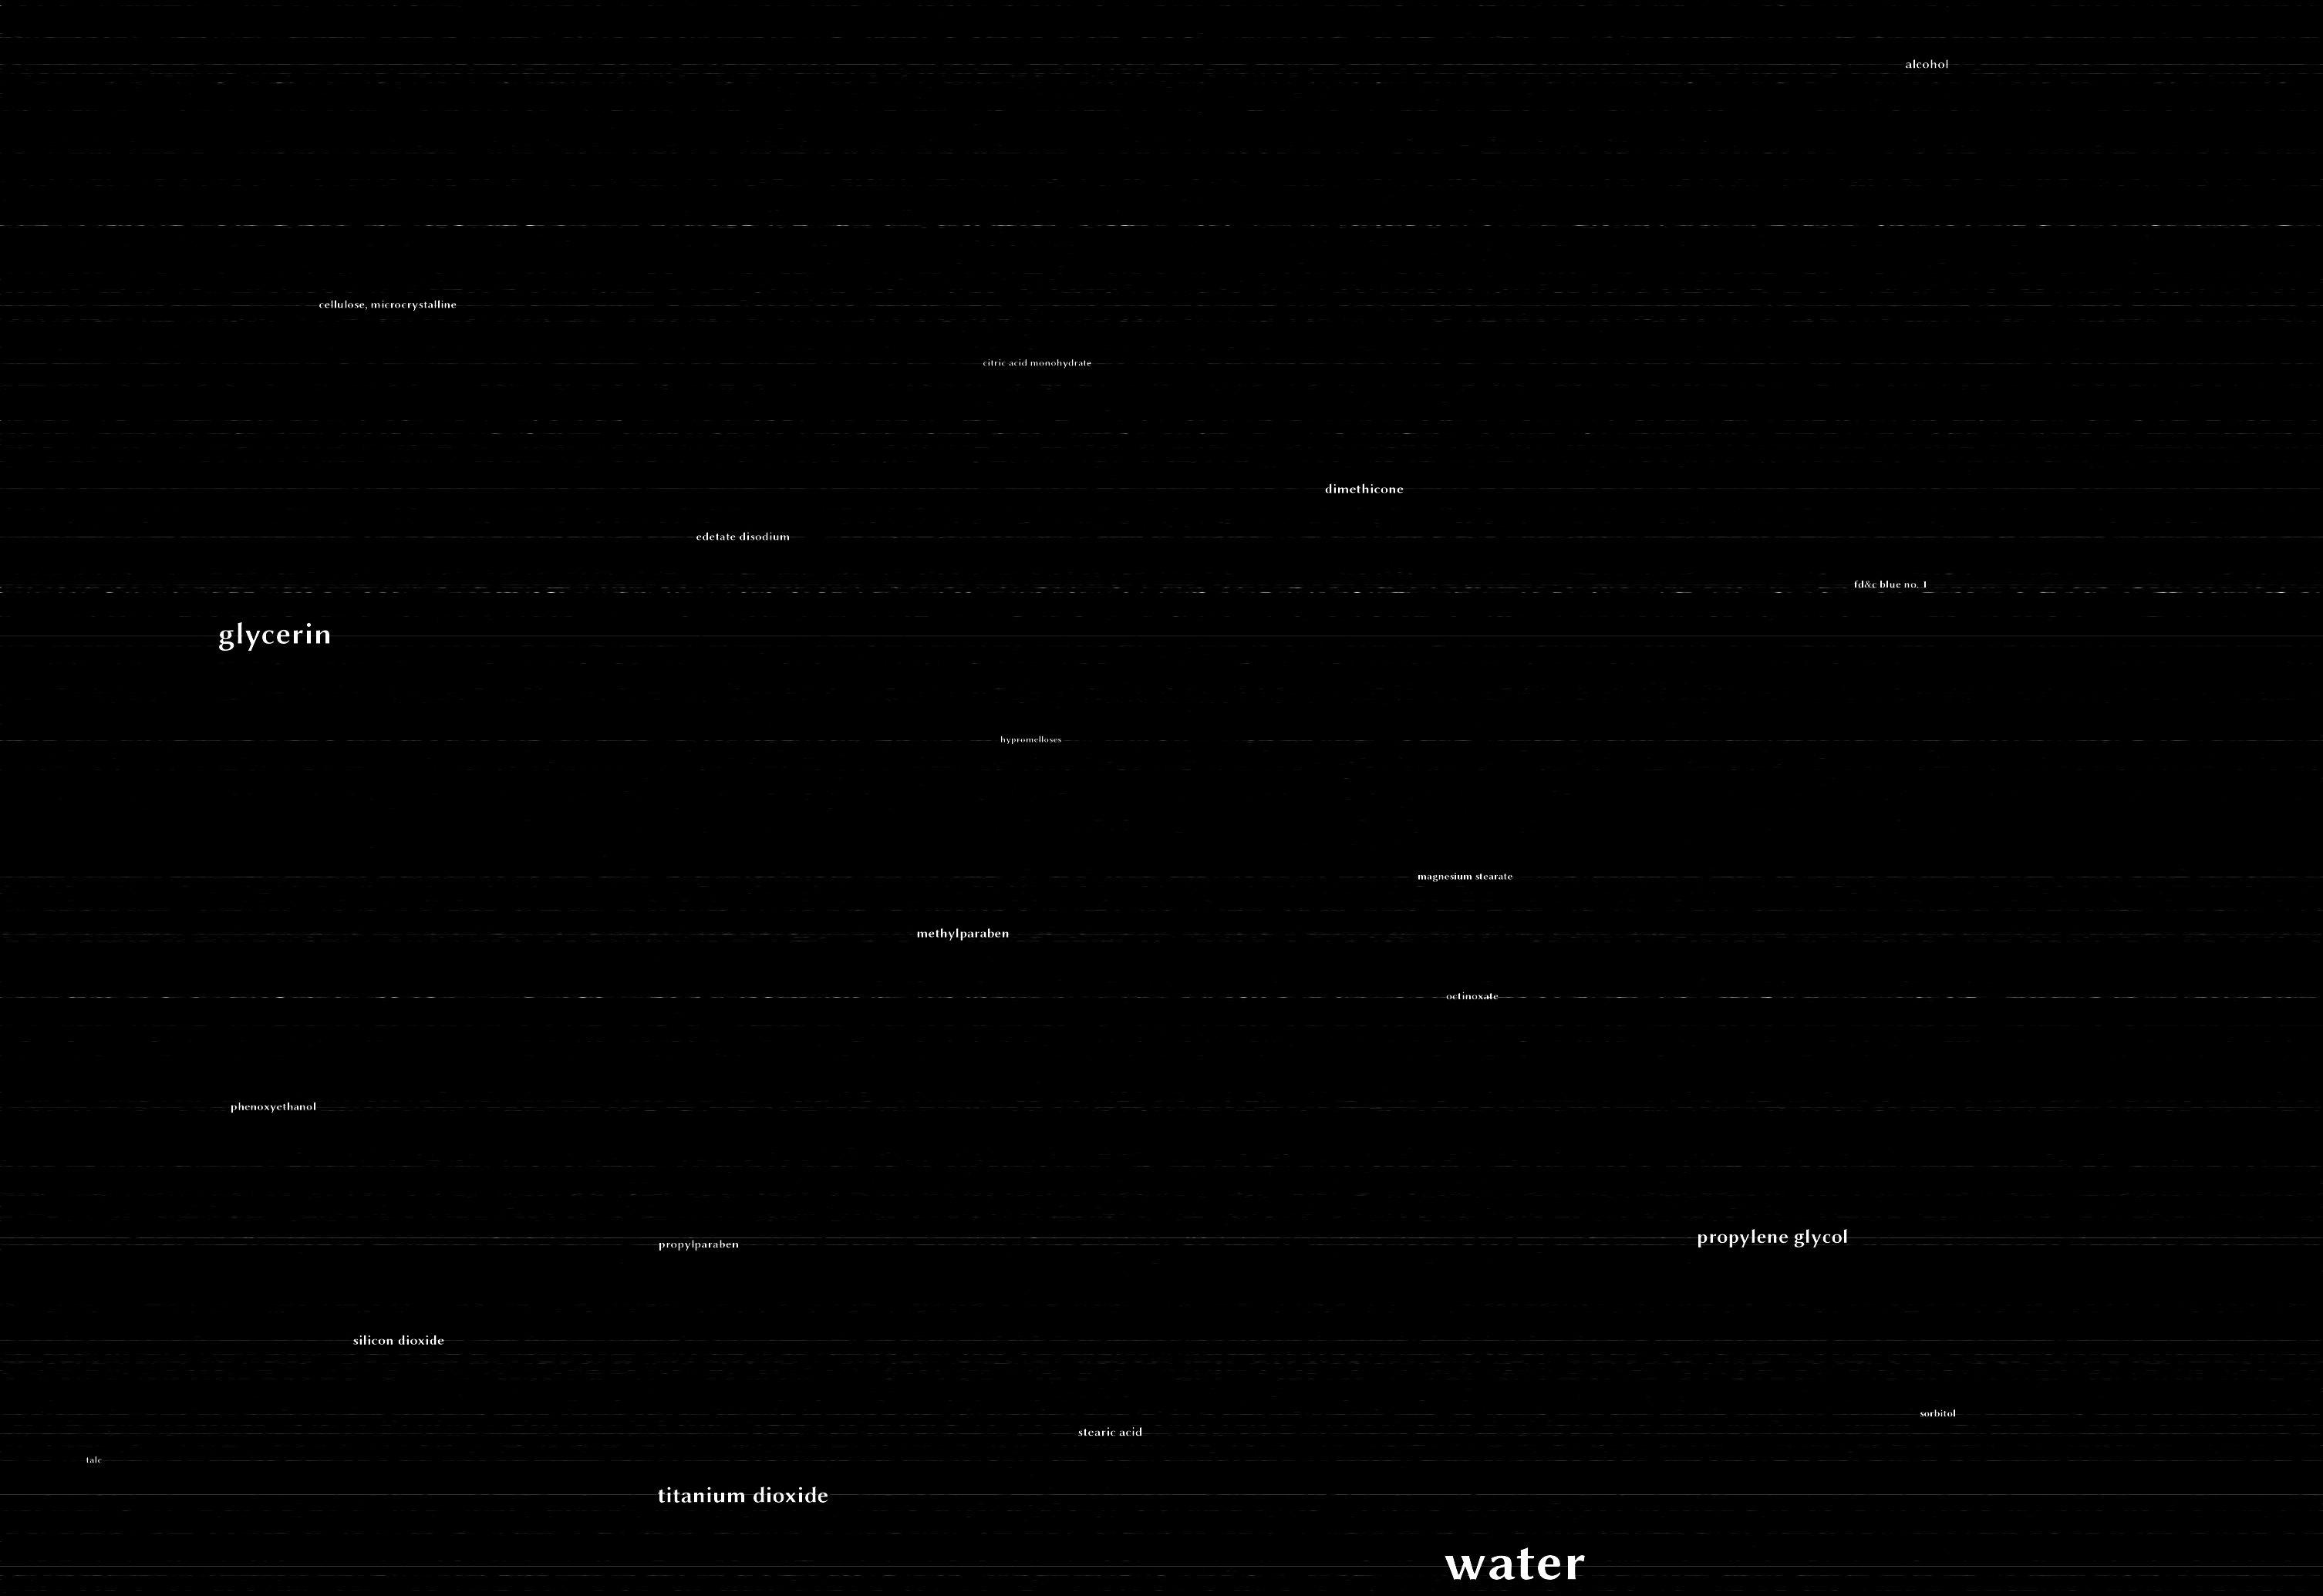
\includegraphics[height=\textheight,keepaspectratio]{drugs}
	\caption{drugs spectrum}
	\label{fig:drugs}
\end{figure}

The most common way to handle this data set would be the usage of a pattern miner, because the data table has only binary entries. I decided to use this data set nevertheless, because the dimensions have very good descriptions and I am able to explain subspaces.

To convert this data to a legal input data set, it is processed as followed: The only preprocessing that is done is to reduce the ingredients to their lower case text because the data set contains the same ingredients written in different combinations of lower and upper case letters. After the case normalization build a list of all ingredients in all drugs and bring them into a fixed order. Every ingredient forms one dimension. Then build a binary vector for every drug in the database where $1$ describes that a ingredient is contained in the drug and $0$ if this is not the case. I provide a parser and converter for this kind of data.

GraBaSS is used with $t_e = 0.25$, $t_n = 0.65$ and $d = 3$. It extracts many subspaces, that describe rare combinations, that are used in some natural products. The listed substances are also natural, e.g. leafs, flowers and roots. Because the ingredients are so uncommon, they form subspaces when only used together only a few times. To handle this issue, the ingredients are sorted according to the number of drugs that uses them and the upper quarter is picked. For this reduces data set, GraBaSS finds subspaces like this: 
\begin{itemize}
	\item alanine; arginine; glycine; methionine; phenylalanine; proline; thrionine
	\item citronellal; d\&c orange no. 5; d\&c red no. 6, 7, 21, 30 and 36
	\item barium, calcium, ethylene, iron, isopropylparaben, sulfate ion
	\item avobenzone; homosalate; octisalate; octocrylene; oxybenzone
\end{itemize}

ENCLUS extracted very small subspaces. When increasing $\epsilon$, the algorithm does not finish within hours because the data set is too large. So I got no usable results.

\section{Tests with outliers}

\begin{table}
	\caption{Test results}
	\label{tab:tests}
	\centering
	\begin{tabular}{lrrrrr}
		\toprule
		\textbf{Data set} & \textbf{GraBaSS} & \textbf{ENCLUS} & \textbf{PCA} & \textbf{Random} & \textbf{Fullspace} \\
		\midrule
		pendigits & \textbf{\num{0.62}} & \num{0.52} & \num{0.43} & \num{0.55} & \num{0.55} \\
		mutant & ? & -- & ? & ? & ? \\
		energy & ? & -- & ? & ? & ? \\
		\bottomrule
	\end{tabular}
\end{table}

\section{Timing}\label{sec:time}

\begin{table}
	\caption{Timing in seconds}
	\label{tab:time}
	\centering
	\begin{tabular}{lr}
		\toprule
		\textbf{Phase} & \textbf{mutant} \\
		\midrule
		Binning & \num{80.7} \\
		Pre-calculation & \num{0.6} \\
		Graph build-up & \num{893.0} \\
		Graph fixing & \num{0.2} \\
		Clique searcher & \num{1.4} \\
		\midrule
		Total & \num{976.1} \\
		\bottomrule
	\end{tabular}
\end{table}
